% @author Arian Helberg

\chapter{Implementierung}

Zur Umsetzung der vorgestellten Konzepte wird im Folgenden auf Softwarepakete, Technologien, Datenspeicherung,
Benutzerinteraktion und Arbeitsablauf der erstellten Software eingegangen.
Darüber hinaus wird ein Überblick über genutzte Hardware und einige Implementierungsentscheidungen gegeben.
Auf Implementierungsdetails zur Nutzung der vorgestellten Technologien wird nicht eingegangen.

\section{Projektstruktur}
Das Softwareprojekt ist nach der Gradle-Source-Code-Konvention organisiert.
Das gesamte Programm befindet sich im Ordner Generator, der obligatorische Gradle-Dateien und den
Source-Ordner enthält.
Sowohl die Quelldateien, also auch die Testdateien sind der Paketstruktur \textbf{de.haw} untergeordnet.
Die folgende Tabelle gibt einen Überblick über grundlegende Pakete und deren Funktion.

\begin{figure}[H]
    \centering
    \begin{tikzpicture}
        \draw[color=black!60!white]
        \FTdir(\FTroot,root,Generator){
            ++(0,-0.2em)
            \FTdir(root,src,src){
                ++(0,-0.2em)
                \FTdir(src,main,main){
                    ++(0,-0.2em)
                    \FTdir(main,java,java) {
                        ++(0,-0.2em)
                        \FTdir(java,de,de) {
                            ++(0,-0.2em)
                            \FTdir(de,haw,haw) {
                                ++(0,-0.5em)
                                \FTdir(haw,gui,gui) {
                                    ++(0,-0.5em)
                                    \FTdir(gui,shape,shape) {}
                                    ++(0,-0.5em)
                                    \FTdir(gui,structure,structure) {}
                                    ++(0,-0.5em)
                                    \FTdir(gui,template,template) {}
                                    ++(0,-0.5em)
                                    \FTdir(gui,turtle,turtle) {}
                                }
                                ++(0,-0.5em)
                                \FTdir(haw,lsystem,lsystem) {}
                                ++(0,-0.5em)
                                \FTdir(haw,pipeline,pipeline) {
                                    ++(0,-0.5em)
                                    \FTdir(pipeline,pipe,pipe) {}
                                }
                                ++(0,-0.5em)
                                \FTdir(haw,tool,tool) {}
                                ++(0,-0.5em)
                                \FTdir(haw,tree,tree) {}
                                ++(0,-0.5em)
                                \FTdir(haw,tree,utils) {}
                            }
                        }
                    }
                }

                \FTdir(src,test,test) {
                    \FTdir(test,java,java) {
                        \FTdir(java,de,de)
                    }
                }
            }
        };
    \end{tikzpicture}
    \caption{Softwareprojekt Dateistruktur}
\end{figure}

\begin{figure}[H]
    \centering
    \begin{tabular}{l|l}
        \textbf{Paket} &  \textbf{Funktion} \\ \hline
        \textit{gui} & Visualisierung des Programms \\ \hline
        \textit{lsystem} & L-System-Repräsentation \\ \hline
        \textit{pipeline} & Umsetzung des Pipeline-Design-Patterns \\ \hline
        \textit{tool} & Methodiken und Algorithmen \\ \hline
        \textit{tree} & Komponenten der Baumstruktur \\ \hline
        \textit{utils} & Hilfskomponenten
    \end{tabular}
    \caption{Softwarepakete mit zugehörigen Funktionen}
\end{figure}

\section{Technologien}
Zur Umsetzung des Softwarepojektes wird eine Java-Anwendung für die Java-Laufzeitumgebung entwickelt.
Sie liegt in der Distribution \textbf{Amazon Corretto} in der Version 11.0.3\_7 vor.
Grafische Oberflächen werden mit der JavaFX-Spezifikation von Oracle in der Version 11.0.2 umgesetzt.
Zur Automatisierung von Abhängigkeits- und Buildmanagement wird Gradle (Version 6.7) verwendet.
Eine Testumgebung, eine Vektorbibliothek, eine Tupelrepräsentation und eine Erweiterung zur mathematischen
Standartbibliothek werden über Abhängigkeiten vom Gradle-Framework im Build-Prozess geladen und zur Verfügung
gestellt.\\
Um den test-driven Implementierungsansatz umzusetzen wird JUnit 5 Jupiter als Testumgebung genutzt.
Sie setzt sich aus einem Programmierschema und einem Erweiterungsmodell zusammen.
Das Jupiter-Projekt liefert zudem die Laufzeitumgebung für Softwaretests.
Googles Guava liefert eine Bibliothek mit mathematischen Funktionen.
Sie wird benötigt, um eine praktikable Lösung zu Mengenmanipulation nutzen zu können (Bsp. Erstellen
von Kombinationspaaren einer Menge).
Ausschließlich JavaFX wird außerhalb des Projektes installiert und als Modul im Start-Skript des Programmes
hinzugefügt.
\\~\\
Weitere Systeme zur Erstellung des Softwareprojektes sind:
\begin{itemize}
    \item Versionierung via Git,
    \item Dot zur Visualisierung von Graphen und
    \item PlantUML zur Generierung von UML-Diagrammen
\end{itemize}

\newpage%TODO: Remove

\section{Konzeptumsetzung}

Das Skript \texttt{Generator.bat}, das zum Starten der Anwendung innerhalb eines Windows-Betriebssystems genutzt werden kann,
fügt dem Programm alle externen Module hinzu, die während der Laufzeit genutzt werden, und führt die angegebene jar-Datei aus:
\begin{csource}
    java --module-path <<Pfad zum JavaFX lib-Ordner>> --add-modules javafx.controls,javafx.fxml,javafx.graphics -jar Generator-0.1.jar
    pause
\end{csource}


Beim Start der Anwendung findet der Benutzer die grafische Oberfläche folgendermaßen vor:
\begin{figure}[H]
    \centering
    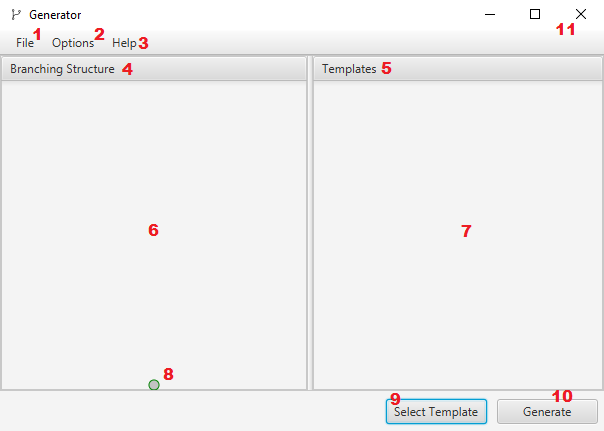
\includegraphics[width=14cm]{../images/UI_numbers.png}
    \caption{Programm nach Ausführung des Start-Skripts}
\end{figure}
Der Menüeintrag \textbf{1} beitet Funktionen zum Laden der vom Benutzer definierten Templates

\subsection*{Visualisierung und Baumstruktur}

\section{Entscheidungen}

\subsection*{Änderbarkeit}
\subsection*{Risiken}
\subsection*{Qualitätsmerkmale}
\subsection*{Alternativen}
\subsection*{Aufwand der Implementierung}